\section{課題4}
課題4のソースコードと実行結果を示す.

\subsection{課題4-1}
\lstinputlisting[caption=kadai4-1.py]{../source/kadai4-1.py}

実行結果は以下の様になった.

\begin{figure}[h]
  \begin{center}
    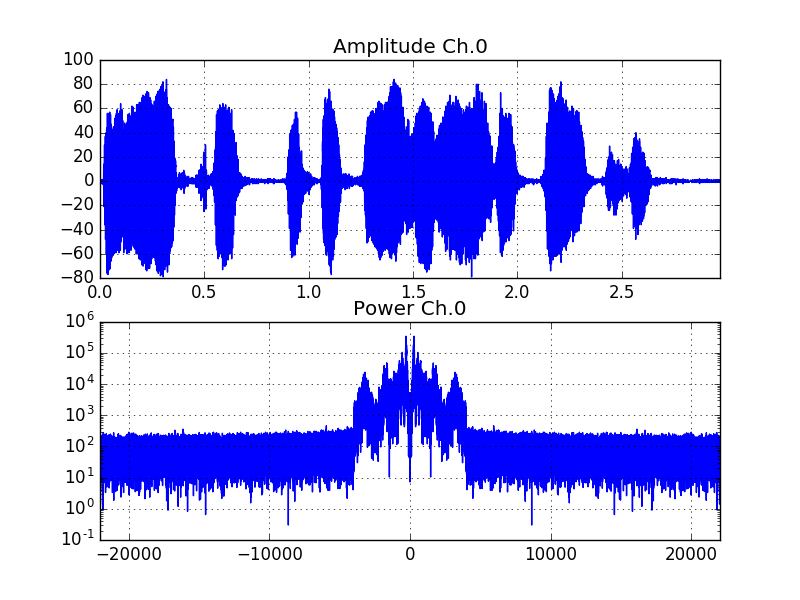
\includegraphics[width=10cm]{./img/kadai4-1-0.png}
    \caption{kadai4-1-0.wav}
  \end{center}
\end{figure}

4000Hzでカットしたため,4000Hz以上のスペクトルが均されている.これはノイズが除去された証拠である.

\begin{figure}[h]
  \begin{center}
    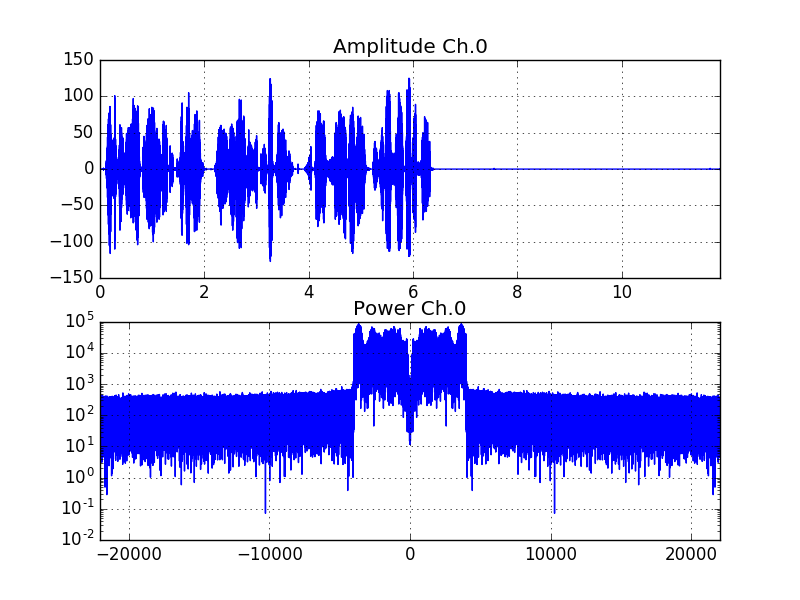
\includegraphics[width=10cm]{./img/kadai4-1-1.png}
    \caption{kadai4-1-1.wav}
  \end{center}
\end{figure}

\begin{figure}[h]
  \begin{center}
    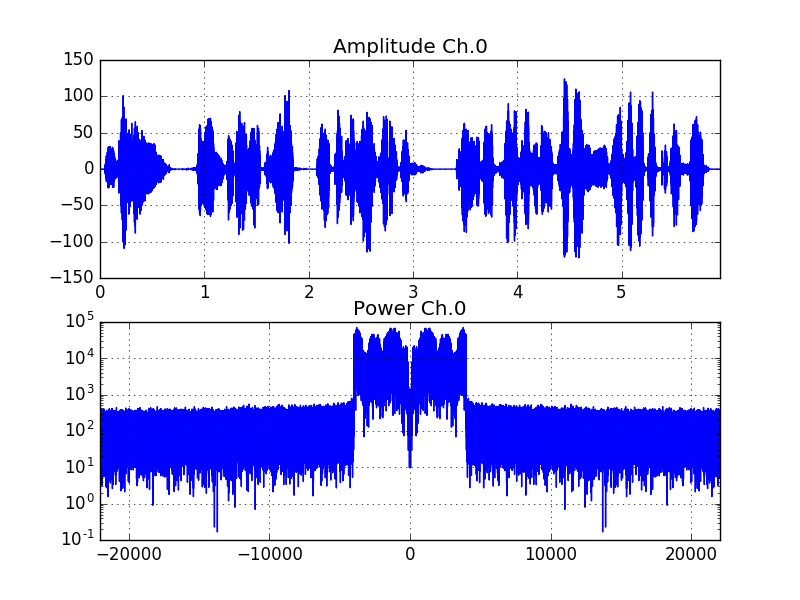
\includegraphics[width=10cm]{./img/kadai4-1-2.png}
    \caption{kadai4-1-2.wav}
  \end{center}
\end{figure}

